% !TeX root = main.tex

% ============================================================
% thesis-sync entry: 2026-07-19_inchworm-intro-concept
% Type: design decision (platform concept) + prior-work integration
% Part of the INCHWORM ROBOT block (prior work, precedes the lizard sections).
% Insertable section block (no preamble). Requires: graphicx.
% ============================================================

\section{OMNIDIRECTIONAL SOFT INCHWORM CLIMBING ROBOT}
\label{sec:inchworm-intro}

The soft actuator and multichannel pneumatics that underpin the
lizard-inspired robot of the later chapters were first developed and
validated on a simpler platform: a single-actuator soft inchworm climbing
robot. This chapter documents that platform. It presents the omnidirectional
bending actuator, its finite-element optimization, its fabrication, the
custom pneumatic driver and controller, and the locomotion gaits that were
demonstrated on an inclined substrate. The three-chambered actuator
introduced here is the direct antecedent of the miniaturized body--tail unit
described in Section~\ref{sec:lizard-architecture}, and the eight-channel
solenoid pneumatic system described in
Section~\ref{sec:inchworm-pneumatics} is specific to this robot.

\subsection{Motivation and Related Work}

Soft robots, constructed from compliant materials, offer inherent impact
resilience that is well suited to climbing applications in confined spaces
such as pipeline interiors~\cite{Gu2018SoftWallClimbing}. Navigating such environments
requires the ability to transition between surfaces meeting at varying
angles. A fundamental challenge for this capability is the transition from a
horizontal plane to an inclined or vertical surface, the so-called
floor-to-wall transition. State-of-the-art designs, however, often lack the
vertical-plane mobility required to execute these maneuvers. Inchworm-inspired
soft robots such as those proposed by Qin et al.~\cite{Qin2019Versatile} and
Hu et al.~\cite{Hu2023Inchworm} use parallel actuator configurations to
achieve steering, but remain predominantly limited to locomotion on
continuous flat planes and lack the adaptability to negotiate intersecting
surfaces or sharp corners.

To address this limitation, a novel soft inchworm robot was proposed,
composed of a single fiber-reinforced cylindrical actuator with a tri-axial
chamber cross-section. This geometry enables omnidirectional bending,
providing both the planar maneuverability and the vertical mobility required
to perform floor-to-wall transitions. Exploiting the fact that the actuator
is pneumatically powered, the robot employs two suction cups located at the
distal ends of the actuator as its surface-anchoring mechanism.

\subsection{Design Concept and Locomotion Gait}

Fig.~\ref{fig:inchworm-concept} illustrates the robot's design concept and
the four phases of its fundamental locomotion gait, which is based on a
coupled combination of bending and elongation. Unlike conventional
inchworm architectures that contract and extend along a single axis, the
present robot advances by bending the actuator to draw one extremity forward
and then elongating it to advance the other, so that the same
three-chambered actuator produces both the propulsive stride and the
directional control.

To ensure that the feet remain strictly parallel to the crawling surface
during Phases~1 and~3 of the gait, a soft hinge-like structure was
integrated into the design. This compliant joint enables the feet to
passively rotate relative to the actuator's extremities, maintaining
consistent and reliable surface adhesion throughout the locomotion cycle.

\begin{figure}[tbh]
  \centering
  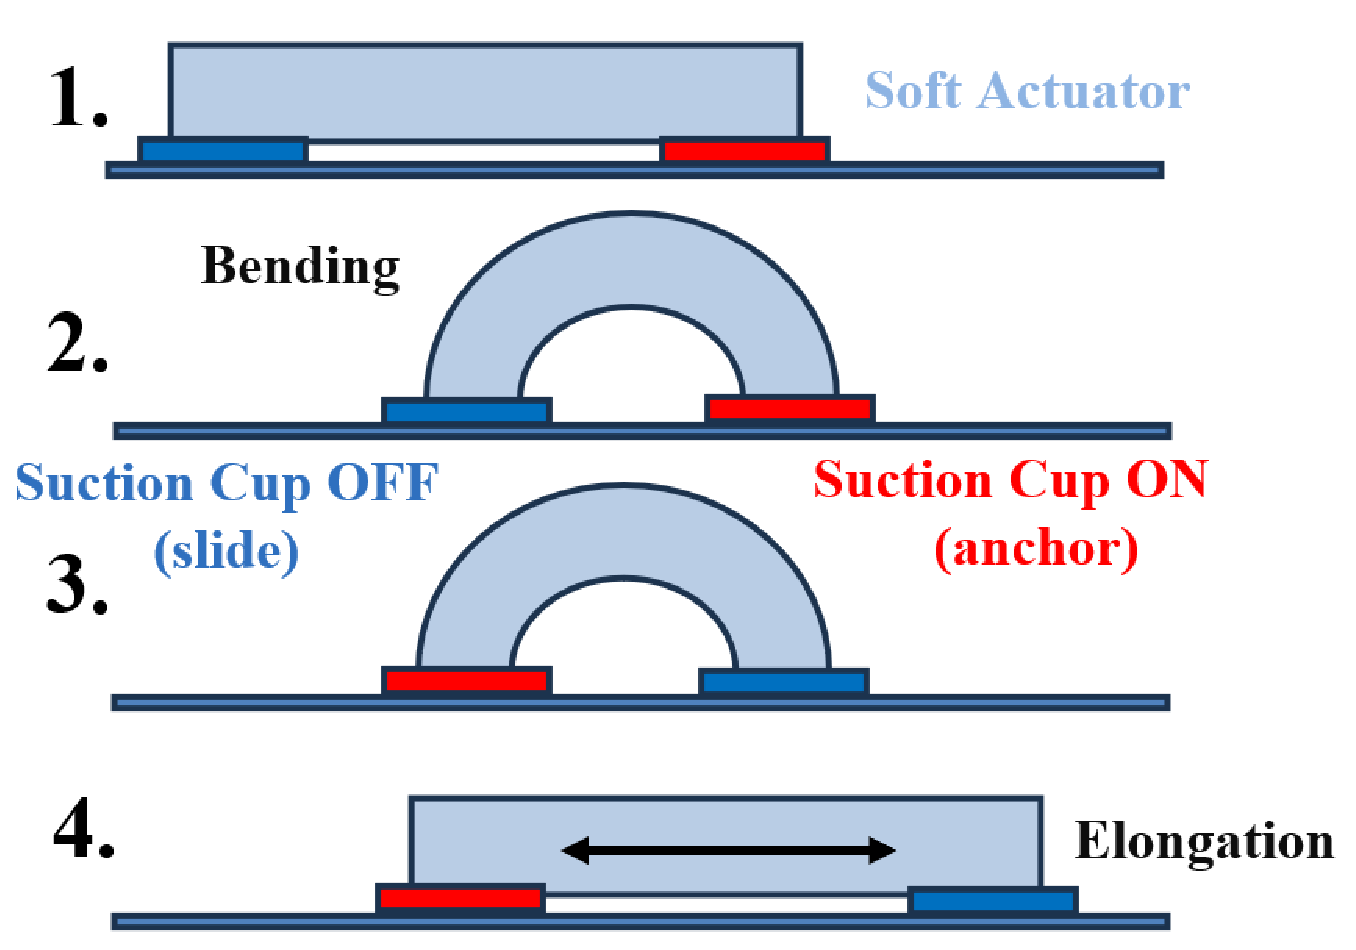
\includegraphics[height=38mm]{figures/concept.eps}
  \vspace*{-2mm}
  \caption{The soft inchworm robot's design concept and fundamental gait
  phases. The single three-chambered omnidirectional actuator carries a
  suction cup at each extremity through a soft passive hinge; forward
  locomotion couples bending (to draw the posterior foot forward) with
  elongation (to advance the anterior foot).}
  \label{fig:inchworm-concept}
\end{figure}

\begin{figure}[tbh]
  \centering
  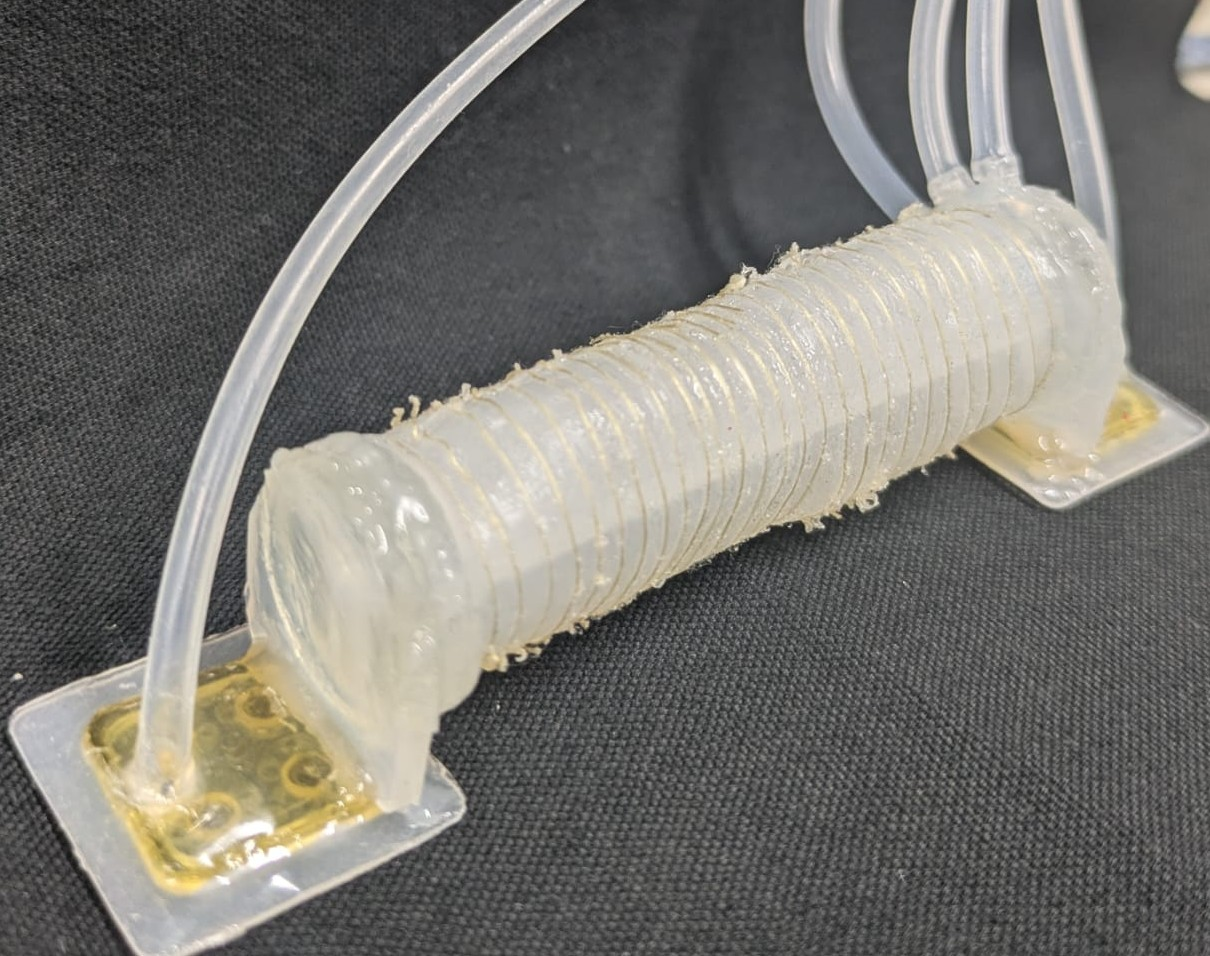
\includegraphics[width=0.95\columnwidth]{figures/InchwormFront.jpeg}
  \vspace*{-1mm}
  \caption{The fabricated soft inchworm robot: a single fiber-reinforced
  three-chambered silicone actuator terminated at each extremity by a
  suction-cup foot bonded through a soft passive hinge, with the pneumatic
  supply tubing routed to the chambers and the cups.}
  \label{fig:inchworm-photo}
\end{figure}
